\documentclass[12pt,oneside,final]{fithesis2}
\usepackage[english]{babel}
\usepackage[utf8]{inputenc}
\usepackage[T1]{fontenc}
\usepackage[backend=biber,sorting=none]{biblatex}
\usepackage[plainpages=false,pdfpagelabels,unicode]{hyperref} %hidelinks
\usepackage[final]{graphicx}
\thesistitle{Mobile Access to jBPM Console}
\thesissubtitle{Bachelor thesis}
\thesisstudent{Tomáš Livora}
\thesiswoman{false}
\thesisfaculty{fi}
\thesisyear{2014}
\thesisadvisor{RNDr. Adam Rambousek}
\thesislang{en}

\addbibresource{bibliography.bib}

\begin{document}
\FrontMatter
\ThesisTitlePage

\begin{ThesisDeclaration}
\DeclarationText
\AdvisorName
\end{ThesisDeclaration}

\begin{ThesisThanks}
Foremost, I would like to express my gratitude to my technical supervisor Ing. Jiří Sviták for his guidance, valuable comments and time invested in consultations throughout the work.

I would also like to thank my advisor RNDr. Adam Rambousek for helping me with all formal aspects of academic writing.

Another big thanks belongs to the jBPM community, especially to the jBPM core developer Ing. Mauricio Salatino who introduced me to the jBPM Console project and helped me a lot with integrating my work into it.
Without him I would never be able to successfully finish the practical part of my thesis.
\end{ThesisThanks}

\begin{ThesisAbstract}
The aim of the bachelor work is to provide...
\end{ThesisAbstract}

\begin{ThesisKeyWords}
business process, JBoss, jBPM, jBPM Console, mobile application, mobile web
\end{ThesisKeyWords}

\tableofcontents

\MainMatter
\chapter{Introduction}
Nowadays, a rapid growth of the market with smart mobile devices like smartphones or tablets can be noticed.
The parameters of these devices are nearly reaching the performance of classic desktop computers.
Unlike them, the mobile devices also offer comfort of mobility so users have an access to their data and applications whenever or wherever they need it.
However, the burden of this feature is lower comfort while using most of the common applications.
Their graphical user interface (GUI) is often optimized just for standard desktop environments and does not take into account lower screen resolution that is typical for mobile devices.
The other problem is much higher finess of the screen which causes that tiny fonts are usually unreadable without zooming in and also makes it difficult to manipulate with very small control components.

The goal of this thesis is to look through the problematics of developing applications optimized for mobile devices, compare advantages and disadvantages of different approaches and find the optimal solution for the jBPM Console\footnotemark\footnotetext{\url{http://www.jboss.org/jbpm/components/console}}.
The mobile version of this application has been proposed on the website of the JBoss community\footnotemark\footnotetext{\url{https://community.jboss.org/wiki/JbpmProjects}} as a further extension of the jBPM project\footnotemark\footnotetext{\url{http://www.jboss.org/jbpm.html}}.
The thesis deals with analysis, design, implementation and testing of the chosen solution which includes creation of a mobile version of this application with predefined subset of its functions like starting new processes or management of user tasks.
As a part of this thesis the integration test suite was also developed.
The resulting product should become a part of the jBPM Console project.
This work does not aim to make a complex review of the given field and is rather focused on the topics relevant to the implementation part.

The thesis starts with an analysis of different approaches to the mobile applications development.
These are divided into three main categories -- native, web and hybrid -- based on their similar features.
Each category is introduced naming its characteristic features.
Then pros and cons of using the given approach are mentioned and the most suitable use case is outlined.
Next chapter deals with business processes, explains related terms and introduces some commonly used standards.
The motivation for using these processes is given and it is described how they are applied to today's business environment.
Then there is explained how business processes can be automated and how modern enterprise applications based on them are developed.
The following sections introduce business process management (BPM) suite called jBPM.
It is described how its workflow engine works and how can be used by developers of enterprise applications.
Also web-based application jBPM Console for managing business processes which is based on the jBPM engine is introduced.
This chapter describes the application only from the user's point of view.
The underlying services that it is powered by are analysed in the next chapter as a part of the analysis and design of mobile application being developed.
There are also mentioned previous attempts to create mobile version of jBPM Console.
Their results together with other factors are considered while choosing the most suitable way of implementing this project.
An adaptive mobile web application is chosen as the final solution.
Next chapter describes the implementation process.
The technologies used are described and some of the most serious problems that occured during this step are mentioned.
The chapter about testing explains what is the main focus while testing this kind of application.
Both unit testing of GWT components and functional testing by Selenium is performed.
The last chapter is a summary of the work done on this project.
The results are presented and plans for future enhancements are outlined.

The outcome of this thesis is a brief overview of the problematics of developing applications optimized for mobile devices.
This knowledge is applied while implementing a mobile version of jBPM Console.
The output of the practical part is a fully functional mobile web application as well as the related test suite.

\chapter{Mobile applications development}
\label{chap:chapter2}
There are many different approaches to the development of mobile applications.
Each of them with its advantages and disadvantages is suitable for another purpose.
To better understand the differences between these approaches, they can be divided into three categories.

\begin{figure}[ht!]
\centering
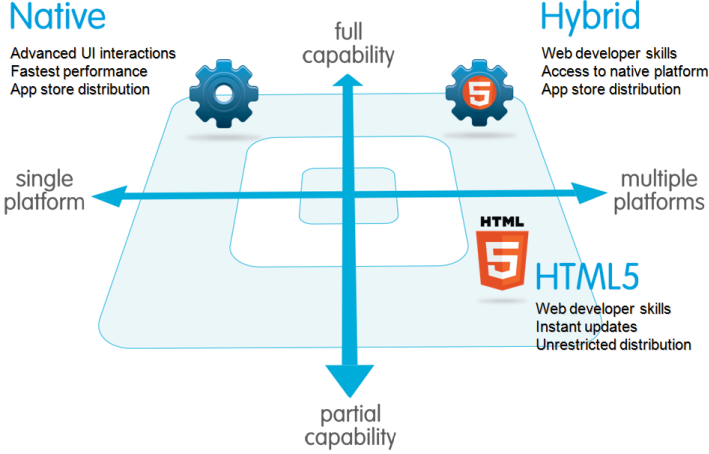
\includegraphics[width=\textwidth]{images/native-html5-hybrid.png}
\caption{Visualization of differences between various approaches to mobile applications development, taken from \cite{developerforce}}
\label{fig:native-html5-hybrid}
\end{figure}

\section{Native applications}
Native applications are designed for the specific platform, e.g. Android, BlackBerry, iOS or Windows Phone.
These applications are installed directly into the target device and are distributed by online markets which are usually platform-specific and offer free as well as paid content.
The examples of such stores are App Store\footnotemark\footnotetext{\url{http://store.apple.com}}, BlackBerry World\footnotemark\footnotetext{\url{http://appworld.blackberry.com}}, Google Play\footnotemark\footnotetext{\url{https://play.google.com/store}} or Windows Phone Store\footnotemark\footnotetext{\url{http://www.windowsphone.com/en-us/store}}.

While developing a native application you have a full access to all the advanced features of the chosen platform like special hardware or operating system-specific functions.
Such software has much better performance than the one created using other approaches because of the lower level of abstraction.
While these applications are distributed by the mentioned markets, they can be easily monetized.
The presence in the market also allows the discoverability of the work of lesser-known authors (or companies) as users can find all applications on one place.
Another advantage of the centralized application market under the control of the company which develops and maintains given platform is that it ensures the quality and safety of the applications.

On the other hand sometimes there may be a conflict between the author's idea of licensing, pricing or updating policy of the application and the rules that must be followed to place the application into the market.
In such cases it is much more difficult to distribute native applications without using the market because the third-part applications are often considered as a security hole and their installation is not allowed by default.
Another problem might be the fact that every platform has its own set of development tools, programming languages and software development kits (SDKs), which make it practically impossible to create cross-platform applications.
This means that a new application needs to be created for each platform which increases the costs of the development proccess.
Users can also use older versions of the application which may bring some additional problems especially when developers add some new functionality to the application that is communicating with the remote devices.
In such cases there is a need for backward compatibility between the different versions.
This may prevent developers from making significant changes and slow down the whole development process.

\section{Mobile web applications}
Mobile web applications are special web pages optimized for mobile devices.
They take into account the limitations and differences of these devices in comparison with desktop computers.
These include smaller screen size, higher fineness of the display, absence of mouse and keyboard, presence of touch control and limited computation power.
But the basic principles of all web pages are also applied in this case.
So you can still find HyperText Markup Language (HTML), Cascading Style Sheets (CSS) and JavaScript on the client's side and the server-side functionality implemented in any suitable language, e.g. PHP, Ruby, Python, Perl or even Java.

The biggest advantage of this approach in comparison with the native applications is that developers do not need to maintain more versions of the application.
This does not only mean that there is one common version for all platforms as users access the application using the web browser.
It also means that all users use the latest version of the application as it is the only one deployed on the server at the time.
This is a significant factor in reducing the development costs as it allows developers not to bother with a backward compatibility so much and make big changes more quickly.
Another important advantage is the fact that developers are not limited by a particular programming language and tools provided for the specific platform.
On the server side they can use any programming language that is supported by the server with any framework or third-part libraries.

However, some new problems might appear when designing mobile web applications.
As users might use various web browsers in different versions there is a need to optimize the application for several versions of all commonly used browsers.
Another thing is the monetizing of this kind of application.
The developers have to set up the advertisements on their own.
They also have to implement their own solution to charge users for using the application.

When designing a mobile web application it is often created as a subset of the funcionality of an existing web application.
In such cases there is usually an intension to somehow connect these two versions to support uniformity and avoid code duplicates.
Nowadays there are basically two ways how to integrate them to one final solution.

\subsection{Responsive web design}
Responsive web design is a technique for developing web applications optimized for different types of devices.
It uses mostly CSS but also JavaScript to adapt the page content to the actual size of the browser's window \cite{marcotte11}.
This technique is suitable when developing a mobile version side-by-side with the full web application.

\subsection{Adaptive delivery}
Adaptive delivery is very similar to the responsive web design.
The main difference is the time when it is decided how the requested page will look like.
While using responsive design it is decided on the client's side by CSS and JavaScript according to the browser's window size, the adaptive delivery is based on different principle.
A type of the client's device is recognized on the server side and only a page for this type of device is sent to the client.
This reduces the amount of incoming traffic on the client side.
It also allows developers to include only relevant parts of the original application in the mobile version.
Some actions might be very difficult to perform on the mobile device so they are likely not to be used and can be ommited from the mobile version.
This approach is prefered to be used also in situations when there is an existing application which is too complex to be changed using the techniques of responsive web design.

\section{Hybrid applications}
Hybrid applications combine the best features of the previous two approaches.
They allow developers to create cross-platform applications that can use some advanced functionality of each platform.
This is achieved by adding another layer which provides JavaScript application programming interface (API) that is common for all platforms.
This API's calls are then translated to native platform-specific API calls.
Such applications are usually written in HTML, CSS and JavaScript.
Then they are packaged as a typical native applications for each platform which means they can be distributed by markets.

The biggest advantage of this approach is that you write only one common code for all platforms.
Developers do not have to learn to use platform-specific tools.
They just get by with the basic web development skills and the knowledge of the provided JavaScript API which allows them to use functions like accelerometer, camera, compass, contacts, file storage, geolocation or notifications.

The drawback of this solution might be the fact that even though you produce applications built for the given platform they do not reach the performance of the native ones.
%\subsection{Web wrapper}
%\subsection{Web-to-native converter}
%\subsection{Native JavaScript API}

\chapter{Business processes and jBPM}
Before designing a mobile version of jBPM Console it is very essential to know what is this application about and how it works.
This chapter explains what business processes are, where they are used and how they can be automated. Also the jBPM engine is introduced and web-based jBPM Console is described both from the users' and developers' point of view.

\section{Business processes}
A business process is a sequence of steps that need to be performed in order to accomplish an organizational goal.
From the technical point of view it can be described as a collection of activities or tasks mutually connected to a logical structure ordered by their time continuity.
Thanks to that a business process can be visualized as a flowchart\footnotemark\footnotetext{A flowchart is a type of diagram used to visualize a process. The individual steps of this process are displayed as various boxes which are connected to each other with arrows determining their order.}.

Nowadays, business processes are so complex and regularly changed that it is practically impossible to hardcode them into the applications and be efficient while adapting to the changes at the same time.
That is why business process management (BPM) tools are used. % BPM vysvetlene uz v uvode
They take control of the maintenance of your business processes and provide API through which your application can easily manipulate with these processes.
This allows developers to focus on the application itself because they do not need to adapt it to the changes in business processes as it is a role of the used BPM tool.

\section{BPMN}
In the past it was usual that every BPM suite implemented and used its own representation of business processes.
As portability became one of the key issues it was necessary to somehow unify these representations and standardize the final outcome so users would be able to reuse their business processes across different BPM tools.

This is why Business Process Model and Notation (BPMN), a standard maintained by the Object Management Group (OMG), was created.
The latest version, BPMN 2.0, is both a business-friendly diagramming notation and an executable process language \cite{silver11}.
The graphical notation of business processes is very similar to activity diagrams from Unified Modelling Language (UML).
A process model is stored as an Extensible Markup Language (XML) file which besides diagram description contains also other information about the process like its data, messages, task assignments etc.

\begin{figure}[ht!]
\centering
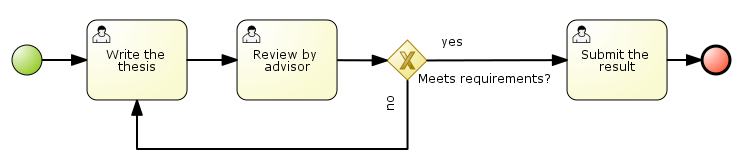
\includegraphics[width=\textwidth]{images/process-example.png}
\caption{Simple example of a business process in BPMN 2.0}
\label{fig:process-example}
\end{figure}

\section{jBPM}
jBPM is an open-source BPM suite developed by the JBoss community \cite{jbpm6overview}.
It can be used to easily model, execute and monitor business processes throughout their life cycle.
The core of jBPM is a light-weight workflow engine that allows users to execute business processes described using the BPMN 2.0 specification.
It can be both embedded in an application or run as a service which users can make use of through the remote APIs.
Besides the core engine, jBPM project also includes other components like a web-based workbench which provides graphical user interface (GUI) for complex management of business processes and Eclipse\footnotemark\footnotetext{\url{https://www.eclipse.org/}} tooling for modeling, testing and debugging of processes.

\subsection{Core Engine}
\label{subsec:core-engine}
The core jBPM engine provides KIE\footnotemark\footnotetext{KIE stands for Knowledge Is Everything.} API to control the execution of business processes \cite{jbpm6api,jbpm6engine}.
To start working with processes it is first necessary to set up Runtime Environment.
The most important thing here that needs to be specified is a list of process definition files.
These definitions are parsed and stored in a form which allows fast automated execution.
After that Runtime Manager, which is resposible for delivering instances of Runtime Engine, can be created.
Runtime Engine encapsulates the two most important elements of the jBPM engine -- KIE Session and Task Service.
KIE Session provides an interface to communicate with the engine.
It allows users to start new processes, manipulate with the running ones or get some information about those that has already finished.

\subsection{Task Service}
The Task Service is a special part of the engine responsible for human task management.
A human task (or user task) is an activity type from BPMN 2.0 specification which needs to be executed by human actor.
Human tasks are used to signalize that users are working on something outside of the system or just to get inputs from them.
Every task is assigned to a specific actor or a group of actors who can claim it and start working on it.
The human task itself has its own life cycle which consists of several states.
The simplified version containing only states relevant to the use cases in jBPM Console is visualized in the figure~\ref{fig:task-lifecycle}.
For a more complex description including all possible states and transitions between them see the jBPM Documentation \cite{jbpm6tasklife} or WS-HumanTask Specification \cite{ws-humantask}.

\begin{figure}[ht!]
\centering
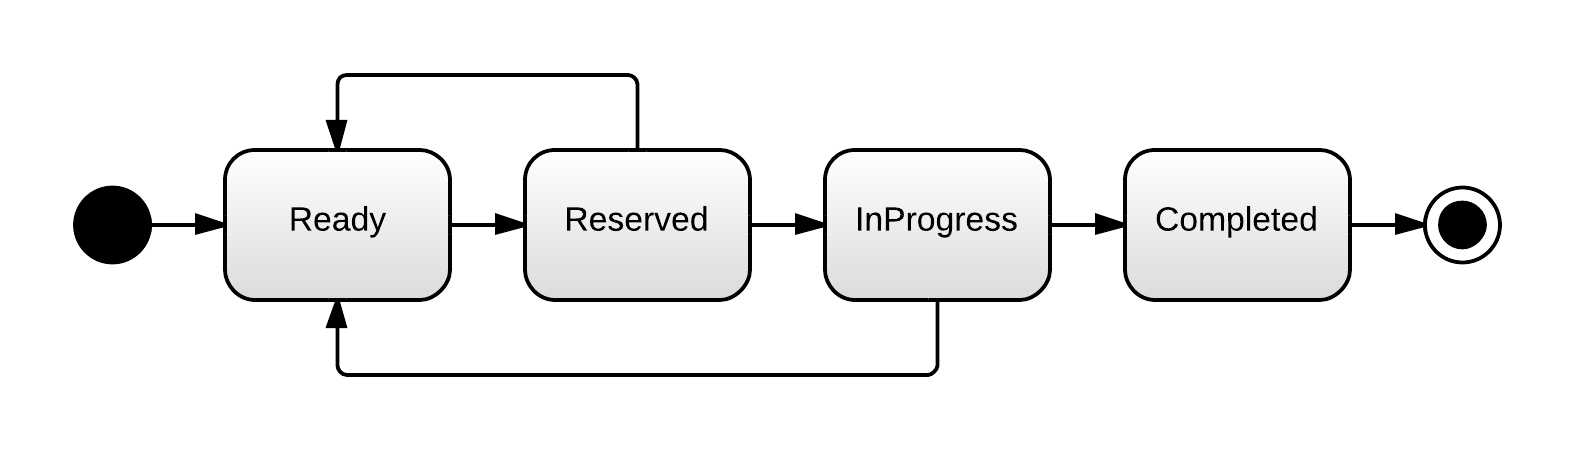
\includegraphics[width=\textwidth]{images/task-lifecycle.png}
\caption{Simplified version of a human task life cycle}
\label{fig:task-lifecycle}
\end{figure}

The Task Service provides a simple API that allows users to handle human tasks.
Using this API tasks can be claimed, started and completed by a user or delegated to someone else.
While completing a task users are able to pass some parameters.
These can be further processed or mapped directly to the process variables.
This is how the interaction between a user and a process instance is ensured and how user actions can influence the following steps in the process execution.

\section{jBPM Console}
The jBPM Console is a web-based tool built on the top of the jBPM services.
It is composed of several components like Guvnor, Designer, Form Modeller and Dashboard.
All this projects grouped together form one unified environment for assets management, business process modeling, managing process runtime and business activity monitoring.

\begin{figure}[ht!]
\centering
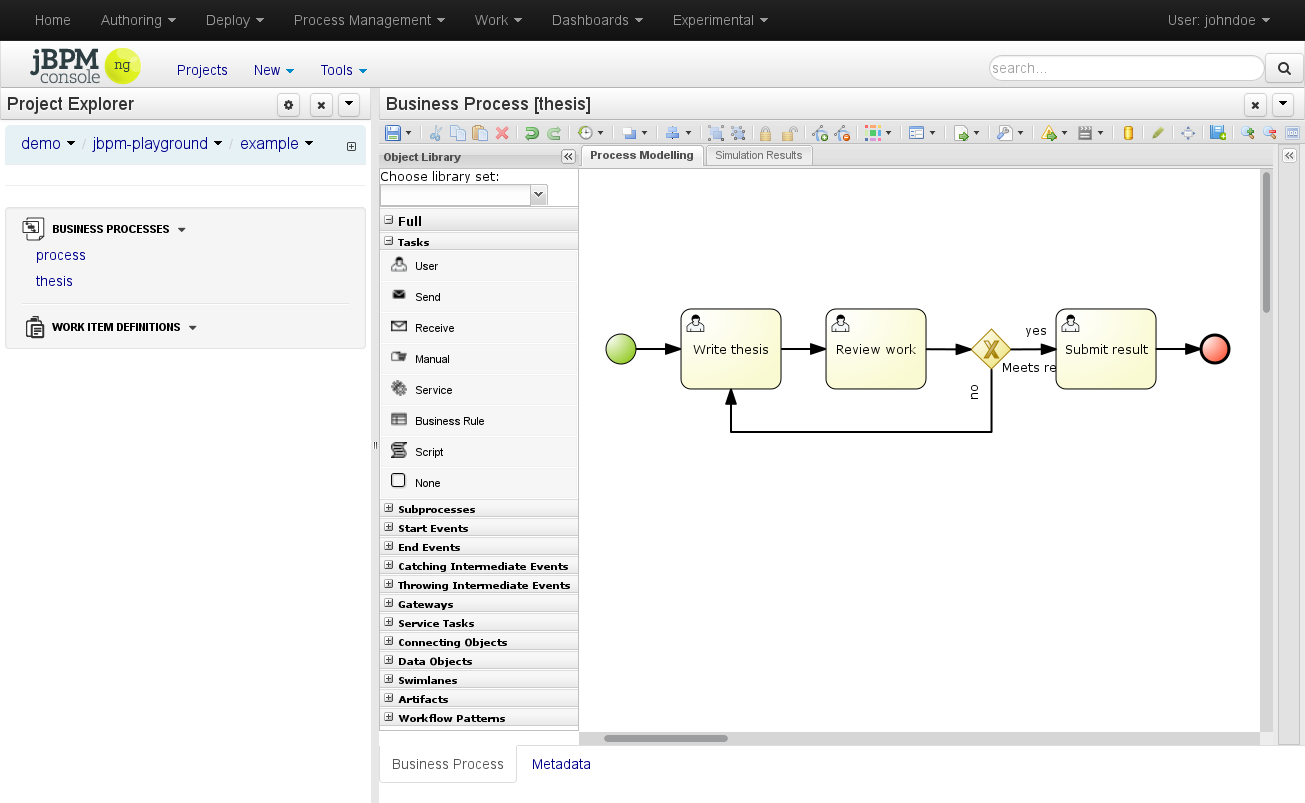
\includegraphics[width=\textwidth]{images/jbpm-console.png}
\caption{Process designer in jBPM Console}
\label{fig:jbpm-console}
\end{figure}

\subsection{Graphical User Interface}
The GUI of the jBPM Console consists of several perspectives.
Each one of them represents one step in the process life cycle.

Authoring perspective is based on the Guvnor component and allows users to manage business assets.
Individual files are stored in Git\footnotemark\footnotetext{Git is a distributed version control system. \url{http://git-scm.com/}} repositories on which a virtual file system (VFS) is based.
%These repositories are organized into bigger structures called organizational units.
Users can create a new repositories or clone the remote ones.
Maven\footnotemark\footnotetext{Maven is a software project management tool. \url{http://maven.apache.org/}} projects are created inside these repositories to simplify organization of the files.
Within these projects several types of new files can be created from which the most important are business process definitions in BPMN 2.0 format and task as well as process forms.
Processes can be edited in their graphical representation by the Designer.
This editor allows users to easily model business processes using the drag\&drop.
After the editing is done a project can be built and deployed so the individual processes within it become ready to be started.

All deployed projects can be seen in a list which is a part of the Deploy perspective.
Users are able to undeploy these projects or create a new deployment unit.

Processes from the deployed projects are all listed in the process definitions list which is a part of the Process Management perspective.
For each process definition there are options to start it as a new process, view its flowchart representation or view all of its instances.
If a process is started a user is prompted to fill in the process form which consists of some input fields.
%if there are any defined.
These inputs are used to initialize process variables.
All process instances are listed in the process instance list where they can be easily controlled.
A running process can be aborted or a signal can be sent to it by a user.
The history of the process variables can also be viewed here.

The Tasks perspective is the one responsible for human tasks management.
Users can view all the tasks that belongs to them or to the groups they are members of.
These tasks are usually created as a result of business process execution but users are also able to create their own personal tasks which do not participate in any process.
Several actions can be executed on these tasks like claiming the ones that nobody is working on, starting work on the claimed tasks and completing tasks.
%Form Modeller

From all the perspectives mentioned above the Process Management and Tasks are the only one that will be included in the mobile version.

\subsection{Modular approach}

From the developer's point of view jBPM Console is a modular application.
Easily said almost every perspective is one independent module.
This approach allows developers to combine modules from different projects and create new applications based on current needs without code duplication.
A typical example is KIE Workbench which is basically jBPM Console merged with Drools Workbench.
The result is a complex application for business processes and rules management with some additional functionality like remote access to its services.

%\subsection{Remote access}


\chapter{Analysis and design}
To be able to design the right solution for the mobile version of the jBPM Console it is essential to compare pros and cons of different approaches to mobile applications development (described in chapter~\ref{chap:chapter2}) with the requirements of the application being developed.
Then some previous solutions for implementing a mobile version of this application are mentioned and their weaknesses are discovered.
Finally, a solution is drafted which is considered to be the most appropriate according to the previous findings.

\section{Possible options}
There are basically two options how a mobile version of the jBPM Console can be implemented.
Both solutions assume that there is an instance of the jBPM Console or KIE Workbench running on the server and the main difference between them is the way how mobile devices communicate with it.

\subsection{Native and hybrid applications}
Although native and hybrid applications are two slightly different approaches to mobile application development in this context there is almost no difference between them.
What is relevant for designing a mobile version of jBPM Console is the environment in which it will run.
Both types of applications run directly on mobile devices.
The only difference is in the development process.
While native applications need to be developed separately for each platform there is only one common code of a hybrid application which is then compiled for each platform.

While these applications run directly on mobile devices there is a need to communicate with KIE Workbench remotely.
This can be achieved by using the REST\footnotemark\footnotetext{Representational state transfer (REST) is an architectural style which uses HTTP commands to execute different actions on resources provided by the server \cite{fielding20}.} API it provides.
Using this interface a client application can execute all common operations with processes or human tasks.
There is practically no difference between executing them via the web GUI of the jBPM Console or using REST calls as the same backend services are called in both cases.

However, this solution has some serious drawbacks.
Not everything can be executed using the REST API.
If there is a need to perform some more complicated commands this interface will have to be extended.
Also every change to the API urges developers to modify all platform-specific clients.

\subsection{Web application}
\label{sec:webapp}
The jBPM Console itself is a web application.
That means if a mobile version is also a web application it might be directly a part of the jBPM Console.
The maintenance of such solution will be much easier than managing several platform-specific clients.
There is also no problem with the limited interface as in this case the mobile version will have access to the same resources as the original application.
This solution can be also divided into two slightly different approaches.

Responsive web design is the first one.
This approach would require completely refactor all existing pages and change their layout to follow the rules of responsiveness.
In such a big application as jBPM Console this will be a very complicated process requiring a lot of effort and with uncertain result.
In addition, not all the parts of the original application are suitable for mobile devices.
Actions performed on some of them might be quite unpractical to do on these devices.

On the other side, adaptive delivery is an approach when the detection is performed on the server side.
This allows to create completely different screens for mobile and desktop users.
jBPM Console is implemented using the Model–view–presenter (MVP) pattern so there is an option to add new implementations of view interfaces optimized especially for mobile devices.

\section{Previous attempt}
Last year there was an attempt to implement a mobile version of jBPM Console \cite{petovsky13}.
At that time the jBPM 6 was just being developed and no stable build of that version had been released so the author decided to use more reliable jBPM 5.
He chose to implement his solution as a native application for Android devices.

This application only allows users to manage processes.
There is a process definitions list where all processes from deployed projects can be found.
A user can choose one of them and start a new instance.
For each process definition there is a list of all running instances.
An instance can be either terminated or there is an option to show the BPMN diagram where the current position of process execution is marked.

The opponent of this thesis mentioned some drawbacks of the resulting product in his report.
There was a question why the author developed the solution for only one specific platform.
The opponent suggested it would be more appropriate to create a web application which could be used on a wide range of different devices.
Also a lack of automated testing was reproached in the report.

\section{Suggested solution}
When choosing the right way of creating a mobile version of jBPM Console it is necessary to consider several factors.
The application should be able to run on all major platforms.
The integration with the original application should be as close as possible.
And the effort needed to develop such solution should also be taken into account.

Considering all these factors together with pros and cons of previously mentioned approaches a mobile web application seems to be the right solution.
Native applications do not offer any advantages over the web ones in the context of jBPM Console.
They have rather some disadvantages mentioned above.
The other thing that favors the web approach is the fact that the original application is also web-based so it just needs to be extended.

However, the process of extending this application is not that easy as it seems to be.
Implementing just new views optimized for mobile devices (as described in section~\ref{sec:webapp}) would probably not be enough.
jBPM Console is intended to be used on high-definition wide screens and consists of many various panels all over the screen.
These panels often provides some fundamental functions and thus cannot be ommited.
In the mobile version a new page for each of these panels must be created.

\section{Application architecture}
This section describes more details about the application being developed.
The architecture is described both in written form and using the Unified Modeling Language (UML) diagrams.

\subsection{Use cases}
The application should provide the functionality to manipulate with process runtime and human tasks.
Going more into the detail, users will be able to see the list of available process definitions and for each one of them start a new instance.
They may list all running process instances and abort any of them as well.
The application also allows users to show their tasks, create a new one, claim available group tasks, release them, start working on a task, complete it or delegate it to someone else.

These are all actions peformed by users on a daily basis.
Other functionality of the jBPM Console is not inteded to be a part of the mobile version.
It would be very unpractical to set up projects or design new processes on mobile devices.

\begin{figure}[ht!]
\centering
\includegraphics[width=\textwidth]{images/use-case.pdf}
\caption{Use case diagram}
\label{fig:use-case}
\end{figure}

The roles used in the use case diagram (figure~\ref{fig:use-case}) are the only two out of five user roles available in the jBPM Console which have the right to work with process runtime and human tasks \cite{jbpm6roles}.

\subsection{Screens and navigation}
Considering all use cases mentioned above, the application GUI can be divided into three sections - process definitions, process instances and human tasks.
Home screen is an entry point to all these sections.
The visualization of all screens and the navigation between them can be found in figure~\ref{fig:screens}.

\begin{figure}[ht!]
\centering
\includegraphics[width=\textwidth]{images/screens.pdf}
\caption{Navigation between screens}
\label{fig:screens}
\end{figure}

Process definitions screen contains a simple list of all available business processes.
In comparison with the original jBPM Console, the items of this list only display the name and version of the process.
When selecting one of them users will get to the screen where more detailed information about the process can be found.
This screen also allows users to start a new instance of the selected business process.

Process instances screen contains a list of all running processes.
For each of them the ID and name of the process is only displayed.
More information about the process instance can be found on the details screen.

The third part, human tasks section, consists of three screens -- tasks list, task details and new task.
On the tasks list screen there is a list of all tasks which the currently logged-in user is a potential owner of\footnotemark\footnotetext{In this context a user is a potential owner of the given task when he is explicitly listed as the actor of that task or when he belongs to a group of users which is the task assigned to.}.
The items of this list only contain the ID and name of the task.
All other information can be found on the task details screen where some of the parameters can be changed as well.
This screen also allows users to claim, start, release or complete the task.
The delegation of the task to someone else is possible here, too.

\subsection{Class hierarchy}
When designing class hierarchy of any large scale application it is a good practise to follow a design pattern.
Although a mobile version of the jBPM Console as described in this thesis is not that big, the further development must be taken into account and so it is essential to design it in accordance with some pattern.
While model–view–presenter (MVP) is one of the most popular design patterns for web applications it was decided to adopt it.
This pattern is also used in the original application and fits the best with the used technologies \cite{ramsdale10}.

\begin{figure}[ht!]
\centering
\includegraphics[width=\textwidth]{images/class-diagram.pdf}
\caption{Class diagram}
\label{fig:class-diagram}
\end{figure}

The class diagram (figure~\ref{fig:class-diagram}) is very similar to the visualization of navigation between screens.
When following the MVP design pattern there needs to be a single presenter and the corresponding view for each screen.
All view classes have one common ancestor which defines the uniform look for them.

\subsection{Modules}
The application is divided into three modules.
Core module contains some common classes used by all views.
There are also view and presenter classes for Home screen located in this module.
Process Runtime module includes all views and presenters working with process definitions and instances.
Human Tasks module comprises of classes associated with tasks screens.
All diagrams in this document use specific color for each module.

\chapter{Implementation}
So far the application architecture was only described on the abstract level.
While this kind of view is very important it is also essential to know something about the actual implementation.
This chapter introduces the used technologies, describes the most serious problems that occured during the implementation phase and provides some code samples from the interesting parts of the application.

\section{Technologies}
This section provides a quick overview of used technologies.
Each of them is briefly introduced and then the explanation why it was decided to use it is given.

\subsection{Google Web Toolkit}
Google Web Toolkit (GWT) is a development toolkit for building and optimizing complex browser-based applications \cite{gwtoverview}.
The biggest difference in comparison with other tools is the fact that using GWT developers write their code in Java and it is then compiled to JavaScript.
This brings some benefits when creating large applications as there are lots of advanced tools for development in Java and the language itself compared with JavaScript has some useful features like strong static type-checking and object-oriented design.

It was decided to use GWT because the jBPM Console is based on it and there was a demand to reuse as many components as possible.
To achieve that it is helpful to build the mobile version using the same technologies as the original application.

\subsection{Mobile GWT}
Mobile GWT (MGWT) extends GWT functionality by adding new features which make it easier to develop web applications optimized for mobile devices.
It adds support for touch events, animations and lots of mobile widgets with platform-specific look-and-feel.

There are also other projects with similar capabilities, for example jQuery Mobile wrapper for GWT\footnotemark\footnotetext{\url{https://github.com/jqm4gwt/jqm4gwt}} (jqm4gwt).
But it was decided to use the MGWT despite the fact that jqm4gwt provides richer pallete of widgets.
The main reason is because the leading developer of MGWT has become a member of the GWT Steering Committee and there are intensions to add support for mobile devices to the next major release of GWT \cite{gwtroadmap}.
This means that GWT 3.0 will probably introduce a new widgets very similar to those from MGWT and so it should be quite easy to switch to it.

\subsection{Errai Framework}
Errai is a GWT-based framework for building rich web applications \cite{erraidoc}.
It provides many useful features from which the most important for this project is the client-side integration for CDI\footnotemark\footnotetext{CDI (Contexts and Dependency Injection) is the Jave EE standard (JSR-299) for handling dependency injection.} and remote procedure calls (RPC) for client-server communication.
%CDI programming model within client code
These two things are the main reason why it was decided to use Errai.
There is an intention to re-use some parts of jBPM Console (described later in section~\ref{sec:reused-components}) and thanks to these features it can be done quite easily.
%CDI

\subsection{UberFire}
UberFire is a rich client platform (RCP) that builds on the strengths of GWT and Errai \cite{uberfire}.
It provides flexible layout components, VFS based on Git repositories and pluggable authentication and authorization system.

The only part of the UberFire this project directly use is the identity provider.
However, other parts are second degree dependencies as some re-used components from jBPM Console rely on them.

\section{Re-used components}
One of the main goals during the development of the mobile version of jBPM Console was to re-use as many components as possible.
Since it was decided to use the same technologies, the mobile application is able to call the jBPM services the same way as the original application do.
This section introduces these services, describes how exactly they are called and what is executed in the background.

Basically, all re-used components from jBPM Console described below are designed the same way.
Each of them is a wrapper for several jBPM services.
From the architectural point of view they are all adapters so they provide interfaces different from services they call in the background.
Going more into the detail, they transform database entities returned by jBPM services to data transfer objects (DTOs) which can be serialized and sent over the wire between server and clients.

\begin{figure}[ht!]
\centering
\includegraphics[width=\textwidth]{images/client-server.pdf}
\caption{Client-server communication}
\label{fig:client-server}
\end{figure}

\label{sec:reused-components}
\subsection{DataServiceEntryPoint}

DataServiceEntryPoint is a wrapper for two jBPM services -- RuntimeDataService and BPMN2DataService.
The first one provides methods for getting information about process definitions, process instances and their variables.
The second one can be used to get some basic information about entities, domain objects, data, forms and tasks associated with a particular business process.

\begin{figure}[ht!]
\centering
\includegraphics[width=\textwidth]{images/refresh-instances.pdf}
\caption{Refreshing the list of process instances using DataServiceEntryPoint}
\label{fig:refresh-instances}
\end{figure}

The sequence diagram in figure~\ref{fig:refresh-instances} is showing how DataServiceEntryPoint is used in the mobile application.
This example describes the whole process of refreshing the list of process instances.
The components on the left are compiled to JavaScript and operate on the client side while the components on the right are run on the application server.
The calling of getProcessInstances() method on DataServiceEntryPoint is implemented using RPC.

\subsection{KieSessionEntryPoint}

KieSessionEntryPoint works with two jBPM services -- DeploymentService and RuntimeDataService.
The first one deals with deployment units which are not used in the mobile application.
The second one was described in the previous section.
It may seem like this component does not provide anything more than DataServiceEntryPoint.
But in fact it does not only wrap the jBPM services but makes use of them to provide more complex functionality.
It allows starting new process instances, aborting, suspending and signaling the running ones or changing values of process variables.

\begin{figure}[ht!]
\centering
\includegraphics[width=\textwidth]{images/abort-process.pdf}
\caption{Aborting a process instance using KieSessionEntryPoint}
\label{fig:abort-process}
\end{figure}

The example shown in figure~\ref{fig:abort-process} explains what is performed when abortProcessInstance() method of KieSessionEntryPoint is called.
This component works directly with RuntimeManager, RuntimeEngine and KieSession (described in section~\ref{subsec:core-engine}).

\subsection{TaskServiceEntryPoint}

TaskServiceEntryPoint wraps only a single jBPM service, InternalTaskService, which provides a wide range of methods for working with human tasks.
It is also a simple adapter like DataServiceEntryPoint so it does not add any functionality and just provides remote interface for Task Service.

\begin{figure}[ht!]
\centering
\includegraphics[width=\textwidth]{images/complete-task.pdf}
\caption{Completing a task using TaskServiceEntryPoint}
\label{fig:complete-task}
\end{figure}


Figure~\ref{fig:complete-task} is showing sequence of steps that are executed in order to complete a given task.
Identity provider from UberFire is used to get the name of the currently logged-in user.

\section{Problems}
During the software development process there are always some difficulties that require a lot of time and effort to be resolved.
This section mentions some of the problems that occured during the implementation of the mobile application and describes how they were handled.

\subsection{Place manager}
One of the main issues was about implementing the right solution for moving between the screens.
While the project is divided into several modules that can be re-used independently it was essential not to create unnecessary dependencies just because there is a need to move between the screens from different modules.

Firstly, a presenter that was in charge of the actual view needed to keep instances of another presenters in order to shift to their views.
This simple solution had a lot of drawbacks including the excess dependencies mentioned above.
It was implemented just to speed up the development process and stay focused on more important parts of the application.

Later when some screens had already been created and successfully tested the mechanism of switching between the screens was completely rewritten.
The new solution was inspired by the one used in MGWT Showcase\footnotemark\footnotetext{\url{https://github.com/dankurka/mgwt.showcase}}.
It was based on one common place manager which was used by all the presenters to switch to other screens.
For each screen a new Place class was created to represent it.
When there was a request to change the actual screen a new instance of this class was created.
Besides indicating which screen would be switched to, it could also carry some parameters for the target view.
Although this solution removed the direct dependencies between presenters, the modules were still not independent as presenters needed to use the place classes of other screens.

Finally, it was decided to implement a solution very similar to the one used in the jBPM Console.
It is also based on a place manager but instead of a special class every screen is represented by a string value.
This allows modules to be independant on each other and be able to move between the screens from different modules at the same time.
It is also a preparation for future migration to UberFire.

\subsection{Integration}
\label{subsec:integration}
The application was originally developed in jbpm-mobile\footnotemark\footnotetext{\url{https://github.com/Salaboy/jbpm-mobile}} repository.
At the time when only screens dealing with tasks were implemented the application was able to run independently as it contained all the neccessary components.

However, a problem occured when screens working with processes were added.
It was necessary to deploy a project containing process definitions in order to start working with them.
To do that jBPM Console needed to be deployed on the application server together with its mobile version.
Because these applications were independent but used the same components there were some conflicts which prevented them from being deployed at the same time.

So it was decided to integrate the mobile version directly to the jBPM Console project to avoid this problem.
This step was planned to be performed when the application was completely finished.
But the circumstances forced them sooner to be able to continue with the development.
The project was thus moved to mobile-integration branch of jbpm-console-ng repository\footnotemark\footnotetext{\url{https://github.com/droolsjbpm/jbpm-console-ng/tree/mobile-integration}} as a new module of jBPM Console.
To get to the mobile screens it is now necessary to show the MobilePresenter in a standalone mode.

\section{Licensing}
The project is licensed under the Apache License, Version 2.0\footnotemark\footnotetext{\url{http://www.apache.org/licenses/LICENSE-2.0}}.
It is a free software license that allows users of the software to use, distribute and modify it without being charged.

It was decided to use this license in order to stay compatible with the jBPM Console project which is also licensed under it.
This allows the mobile version to be incorporated into the project.

\chapter{Testing}
Testing is a very important part of a software development life-cycle.
It helps to detect unseen errors and assure that an application is working as expected.
This chapter describes how the mobile application being developed has been tested.
Two different approaches are mentioned -- manual and automated testing.

\section{Manual testing}
Manual testing is the simpliest way how it can be verified that an application works as expected.
There are no special requirements, an application just needs to be built and deployed in a runtime environment.
That is why this approach is mostly used during the development phase of an application life-cycle.
In this section three different ways of manual testing that were used during the development of the mobile application are mentioned -- desktop browsers, physical devices and the Android Emulator.

\subsection{Desktop browsers}
During the development of the application it was mostly tested in desktop web browsers, namely Chromium and Google Chrome.
It is because the application was run in the GWT debug mode which requires the GWT developer plugin to be installed in the browser.
This plugin is only available for desktop browsers.
Although it may seem inappropriate to test a mobile web application in desktop browsers, there is not a big difference in comparison with mobile browsers.
Both Chromium and Google Chrome browsers use WebKit-based layout engine and both Android and iOS default browsers use WebKit so the rendering of the page is practically the same.
There is only difference in the appearance of the application as MGWT uses platform-specific styles by default.

\subsection{Physical devices}
Later when it was possible to deploy the application on an application server it was also tested using physical devices.
Apple iPhone 4S and HTC Desire SV were chosen as representatives of the two most popular platforms, iOS and Android, as they were easily accessible to the author of this thesis.
On each platform the application looks slightly different as MGWT tries to adopt the platform-specific look\&feel.

\subsection{Android Emulator}
The Android Emulator is a mobile device emulator included in the Android SDK\footnotemark\footnotetext{\url{http://developer.android.com/tools/help/emulator.html}}.
It lets programmers develop and test Android applications without using a physical device.
The emulator requires a creation of Android Virtual Devices (AVDs) which can be managed by the AVD Manager.
When setting up a new virtual device, it is possible to specify hardware configuration as well as a version of used Android OS.

The application being developed has also been manually tested using the Android Emulator.
However, there were only several attempts and the emulator has mostly been used in the automated tests (described later in section~\ref{subsec:test-suite}).

\section{Automated testing}
In case of web-based applications, automated functional testing means clicking on the given elements and filling in the forms according to the selected scenario.
It may seem unnecessary to write these kind of tests for fundamental operations while the application is tested manually many times before it is realeased.
However, test coverage of basic functionality really helps to quickly find regressions when a lot of changes are made.
This applies especially for development of large enterprise applications where it is quite likely that a small modification of source code can cause serious problems and there is no time to check everything manually after each change.

\subsection{Selenium}
Selenium is a suite of tools to automate web browsers across many platforms.
Besides other components it includes WebDriver, a tool which makes direct calls to the browser using each browser’s native support for automation \cite{webdriver}.
WebDriver is the name of the key interface against which tests should be written in Java.
The implementing classes are for example ChromeDriver, FirefoxDriver or SafariDriver.
In the past there were also some implementations supporting mobile testing, AndroidDriver and IPhoneDriver.
However, they have moved to separate projects, Selendroid\footnotemark\footnotetext{\url{http://selendroid.io/}} and ios-driver\footnotemark\footnotetext{\url{http://ios-driver.github.io/ios-driver/}}, as they provide more complex functionality and can be used to write tests for native applications on the given platform as well.

\subsection{Selendroid}
Selendroid is a test automation framework for native, hybrid and mobile web applications running on Android OS.
It is based on WebDriver and so allows to control GUI elements of an application the same way as Selenium does.
Selendroid uses platform-specific tools provided by Android SDK.
It can make use of the Android Emulator or a physical device plugged in via USB to run tests on it.

\subsection{Test suite}
\label{subsec:test-suite}
The test suite developed for the mobile version of jBPM Console is based on Selendroid.
All tests are run in a virtual environment of the Android Emulator.
Before each test the emulator is started and the web application is loaded in its web browser.

The suite includes tests for some basic application functionality.
It tries to run a new process instance and check if it appears in the list of all instances.
After that it runs a new instance of another business process and verify if in the list of instances for the given process definition appears only this instance.
The other tests work with tasks.
They try to claim, release, start and complete a task and check if its status is correctly changed after each of these operations.

\chapter{Summary}
The main goal of this thesis was to find the ideal solution for a mobile version of the jBPM Console and implement it.
This was achieved and the work progress is documented in the previous chapters.
The source code of the application as well as the distribution WAR file are attached.

Since the beginning of the development process, all steps were regularly discussed with one of the jBPM core developers, Mauricio Salatino.
This was done in order to ensure that the project would meet the expectations and be accepted by the jBPM community.
As mentioned in section~\ref{subsec:integration}, the mobile application has already been incorporated into the jBPM Console project.
However, it is now only in the mobile-integration branch.
To get to the master branch there needs to be some discussion in the jBPM community and it will probably also need to be approved by Red Hat, the company which is in charge of the project.

Although the basic functionality has been implemented, there are still many ways in which the mobile application can be enhanced.
Besides adding some new screens or extending the existing ones, other changes may also be performed.
For example the application's look\&feel could be improved by applying some nice-looking CSS.
Or it might be optimized also for tablets which offer higher screen resolution than smartphones.
The author of this thesis plans to continue developing the application and implement some of the enhancements mentioned above.

\printbibliography

\end{document}